%%%%%%%%%%%%%%%%%%%%%%%%%%%%%%%%%%%%%%%%%%%%%%%%%%%%%%%%%%%%%%%%%%%%%%
%%%%%%%%%  TEMPLATE IEEE PARA ENTREGA DEL ARTÍCULO FINAL DE  %%%%%%%%% 
%%%% PRÁCTICA DE INGENIERÍA ELECTRÓNICA DE LA UNIVERSIDAD CENTRAL %%%%
%%%%%%%%%%%%%%%%%%%%%%%%    BOGOTÁ, COLOMBIA    %%%%%%%%%%%%%%%%%%%%%%
%%%%%%%%%%%%%%%%%%%%%%%%%%%%%%%%%%%%%%%%%%%%%%%%%%
%%%%   AUTOR: SERGIO ANDRÉS CHAPARRO MORENO   %%%%
%%%%%%%%%%%%%%%%%%%%%%%%%%%%%%%%%%%%%%%%%%%%%%%%%%
%%%%%%%%%%%%%  VERSIÓN 1.0-ENE 2017  %%%%%%%%%%%%%
%%%%%%%%%%%%%%%%%%%%%%%%%%%%%%%%%%%%%%%%%%%%%%%%%%
\documentclass[journal]{IEEEtran}
\IEEEoverridecommandlockouts
%%%%%%%%%%%%%%%%%%%%%%%%%%%%%%%%%%%%%%
%%%%%%%% PRINCIPALES PAQUETES %%%%%%%%
%%%%%%%%%%%%%%%%%%%%%%%%%%%%%%%%%%%%%%
\usepackage{fancyhdr}
\usepackage{graphicx}
\usepackage[utf8]{inputenc}
\usepackage{color}
\usepackage{hyperref}
\usepackage{wrapfig}
\usepackage{amsmath}% http://ctan.org/pkg/amsmath
\usepackage{array}
\usepackage{multirow}
\usepackage{adjustbox}
\usepackage{amsmath}

\usepackage{algorithm}
\usepackage[noend]{algpseudocode}
\usepackage{nccmath}
%\usepackage{anysize}
\usepackage{pgfplots}
\usepgfplotslibrary{external}
\usepackage{bm}

\tikzexternalize
\usepackage{subfigure}
\usepackage{amsfonts,latexsym} % para tener disponibilidad de diversos simbolos
\usepackage{enumerate}
\usepackage{booktabs}
\usepackage{float}
\usepackage{threeparttable}
\usepackage{array,colortbl}
\usepackage{ifpdf}
\usepackage{rotating}
\usepackage{cite}
\usepackage{stfloats}
\usepackage{url}

\usepackage{listings}
\usepackage{color}

\lstset{
  basicstyle=\ttfamily,
  columns=fullflexible,
  frame=single,
  breaklines=true,
  postbreak=\mbox{\textcolor{red}{$\hookrightarrow$}\space},
}

\newcolumntype{P}[1]{>{\centering\arraybackslash}p{#1}} 
\newcommand{\tabitem}{~~\llap{\textbullet}~~}
\newcommand{\ctt}{\centering\scriptsize\textbf} %%\ctt abrevia el comando \centering\scriptsize\textbf
\newcommand{\dtt}{\scriptsize\textbf} 
\renewcommand\IEEEkeywordsname{Palabras clave}


% correct bad hyphenation here
\hyphenation{op-tical net-works semi-conduc-tor} 

\graphicspath{ {Figs/} } 



\newcommand{\MYhead}{\smash{\scriptsize
\hfil\parbox[t][\height][t]{\textwidth}{\centering
\begin{picture}(0,0) \put(-0,-15){
\includegraphics[width=30mm]{cued}} \end{picture} \hspace{6.5cm}
University of Cambridge \hspace{5.3cm} Version 1.0\\
\hspace{6.6cm} Department of Engineering \hspace{5cm} Date 01/22/19\\
\underline{\hspace{ \textwidth}}}\hfil\hbox{}}}
\makeatletter
% normal pages
\def\ps@headings{%
\def\@oddhead{\MYhead}%
\def\@evenhead{\MYhead}}%
% title page
\def\ps@IEEEtitlepagestyle{%
\def\@oddhead{\MYhead}%
\def\@evenhead{\MYhead}}%
\makeatother
% make changes take effect
\pagestyle{headings}
% adjust as needed
\addtolength{\footskip}{0\baselineskip}
\addtolength{\textheight}{-1\baselineskip}
\usepackage{nomencl}
\makenomenclature
\pgfplotsset{compat=1.9}

\makeatletter
\def\BState{\State\hskip-\ALG@thistlm}
\makeatother


\begin{document}

\title{3F8 Coursework: Classification With Logistic Regression Probabilistic Model}

\author{Tom Xiaoding Lu\\
				\textit{xl402@cam.ac.uk}\\
				Pembroke College\\% stops a space
} %\thanks anexa una nota a pie de página donde se puede colocar alguna información sobre la naturaleza del documento.
%%%%%%%%%%%%%%%%%%%%%%%%%%%
%\thanks{El presente documento corresponde al articulo final del proyecto de práctica de ingeniería electrónica 3 presentado en la Universidad Central durante el periodo 2017-1.}
% Comando que indica la generación del título
\maketitle

\begin{abstract}
This coursework investigates the Logistic Classification model. The model is implemented as a binary classifier, and is tested on a set of two dimensional non-linearly separable data points. The effect of under-fitting is observed through only using linear features. Non-linear feature expansion using radial basis functions is performed on the model with F1=92\%.\end{abstract}

\section{Probabilistic Model and Gradient Ascent}
Consider the Logistic Classification model, aimed to classify a dataset $\mathcal{D}\{\mathcal{X}, \mathcal{Y}\}$ consisting of $N$ datapoints. The $n$th datapoint within the corpus is denoted $\{\bm{x}^{(n)}, y^{(n)}\}$, where $\{\bm{x}^{(n)}\in \mathbb{R}^M\}$, where $M$ is the number of datapoint features. $y^{(n)}$ is the binary label to be predicted by the classifier.\\
To incorporate a bias within the model, the inputs are augmented with a fixed unit input $\bm{\hat{x}}^{(n)}=(1, \bm{x}^{(n)})$. The task of classification can therefore be expressed as:
\begin{equation}
    \bm{\hat{y}}^{(n)} =  \bm{\beta^T\hat{x}}^{(n)} = \beta_0 + \sum_{m=0}^M \beta_m x_m^{(n)}
    \label{eq:model}
\end{equation}
In equation \ref{eq:model}, $\hat{y}^{(n)}$ represents the model predication for the $n$th datapoint, $\bm{\beta}$ is the model parameter vector. The probability of the dataset is therefore a product of Bernoulli distributions, with $\sigma$ being a sigmoid function:
\begin{eqnarray}
    \mathbb{P}(\mathcal{Y}|\mathcal{X}, \bm{\beta}) &=& \prod_{n=1}^{N}\mathbb{P}(  y^{(n)}  |  \bm{\hat{x}}^{(n)}  )\\
    &=&  \prod_{n=1}^{N} \sigma(\bm{\beta^T\hat{x}}^{(n)})^{y^{(n)}}(1-\sigma(\bm{\beta^T\hat{x}}^{(n)}))^{1-y^{(n)}}
    \label{eq:liklihood}
\end{eqnarray}
The gradients of the log-likelihood of the parameters $\frac{\partial }{\partial \bm{\beta}} \mathcal{L}(\bm{\beta})$ where $\mathcal{L}(\bm{\beta}) = \log \mathbb{P}(\mathcal{Y}|\mathcal{X}, \bm{\beta})$ are derived. Letting $u = \bm{\beta^T\hat{x}}$:
\begin{eqnarray}
    \mathcal{L}(\bm{\beta}) &=& \log \mathbb{P}(\mathcal{Y}|\mathcal{X}, \bm{\beta}) \\
    &=& \sum_{n=1}^N y^{(n)}\log \sigma (u) + (1-y^{(n)})\log (1- \sigma (u))
\end{eqnarray}
Taking the derivative with respect to a single parameter $\beta_j$, $\frac{\partial }{\partial \beta_j}$ is:
\begin{eqnarray}
   \sum_{n=1}^N y^{(n)} \frac{\partial }{\partial \beta_j} \log \sigma (u) + (1-y^{(n)}) \frac{\partial }{\partial \beta_j} \log (1- \sigma (u))\\
   = \sum_{n=1}^N y^{(n)} A + (1-y^{(n)}) B \label{eq:comp}
\end{eqnarray}
The partial derivatives $A$ and $B$ are computed separately, applying chain rule:
\begin{eqnarray}
    A &=&  \frac{\partial }{\partial \beta_j} \log \sigma (u) = \frac{\partial }{\partial \beta_j} \log K\\
    &=&  \frac{\partial }{\partial K}\frac{\partial K}{\partial u}\frac{\partial u}{\partial \beta_j}\\ \label{eq:sigmoid_dev}
    &=& \dfrac{1}{K}\sigma(u)(1-\sigma(u))x_j^{(n)}\\
    &=& (1-\sigma(u))x_j^{(n)}
\end{eqnarray}
Equation \ref{eq:sigmoid_dev} can be written since the derivative of a sigmoid function is $1-\sigma(u)$. Repeating the same procedure to $B$:
\begin{eqnarray}
    B &=&  \frac{\partial }{\partial \beta_j} \log (1 - \sigma (u)) \\
    &=& \dfrac{1}{K}\sigma(u)(\sigma(u)-1)x_j^{(n)}\\
    &=& -\sigma(u)x_j^{(n)}
\end{eqnarray}
Substituting $A$ and $B$ into equation \ref{eq:comp} the partial derivative with respect to one of the parameters is computed:
\begin{eqnarray}
   \frac{\partial \mathcal{L}}{\partial \beta_j} &=& \sum_{n=1}^N [y^{(n)} - \sigma(\beta^T\hat{x}^{(n)})]\hat{x_j}^{(n)}  \\
   &=& \sum_{n=1}^N [y^{(n)} -\hat{y}^{(n)}]\hat{x_j}^{(n)} \label{eq:grad}
\end{eqnarray}
Intuitively, equation \ref{eq:grad} states that the likelihood gradient with respect to $\beta_j$ equals to the error term $y^{(n)} -\hat{y}^{(n)}$ multiplied by the datapoint's feature $\hat{x_j}^{(n)}$ that the parameter is responsible for, summed over all datapoints in the dataset.\\
Denoting the new parameter vector $\hat{\bm{\beta}}$, the parameter update procedure can therefore be written as:
\begin{equation}
    \hat{\bm{\beta}} = \bm{\beta} + \eta \frac{\partial }{\partial \bm{\beta}} \mathcal{L}(\bm{\beta})
\end{equation}
The parameter update can be done incorporating the vectorized format of equation \ref{eq:grad}, using the dataset matrices $\mathcal{X}$ and $\mathcal{Y}$:
\begin{equation}
     \hat{\bm{\beta}} = \bm{\beta} + \eta \mathcal{X}^T(\mathcal{Y}-\sigma(\mathcal{X}\bm{\beta}))
\end{equation}

The pseudocode implementation of the gradient ascent algorithm is shown in algorithm \ref{algo:grad}.
\begin{algorithm}
\caption{$\beta$ Gradient Ascent}\label{algo:grad}
\begin{algorithmic}[1]
\Procedure{Sigmoid}{$\{x_i\}_{j=1}^N$}
\Return $1/(1 + exp(-x))$
\EndProcedure
\Procedure{Pad\_ones}{$\{x_{i,j}\}_{i,j=1}^{N,M}$}
\State $\{y_{i,j}\}_{i,j=1}^{N,M+1} \gets 0$
\State $\{y_{i,j}\}_{i,j=1,2}^{N,M+1} \gets \{x_{i,j}\}_{i,j=1}^{N,M}$
\Return $\{y_{i,j}\}_{i,j=1}^{N,M+1}$
\EndProcedure

\Procedure{Logistic\_regression}{$X, Y, \text{l\_rate}, \text{max\_iter}$}
\State $\text{loss} \gets [\;]$
\State $X \gets \text{Pad\_ones}(X)$
\State $\bm{\beta} \gets \text{random uniform vector}$

\For{$i < \text{max\_iter}$}
    \State $\text{y\_pred} \gets \text{sigmoid}(X^T \bm{\beta})$
    \State $\text{loss} \gets \text{compute\_average\_loss}(X, Y, \bm{\beta})$
    \State $\bm{\beta} \gets \bm{\beta} + \text{l\_rate} * X^t (Y-\text{y\_pred})$
\Return $\bm{\beta}, \text{loss}$
\EndFor
\EndProcedure

\end{algorithmic}
\end{algorithm}


\section{Exploratory Data Analysis}
As the dimension of the input dataset is two, the exploratory data analysis (EDA) is carried out by simply plotting all data points with axis being the two features, coloured according to the class of the datapoint shown in figure \ref{fig:a}. From the plot, it is clear that to classify the datapoints, a linear boundary is not suitable for this purpose. Non linear transformation on features of the datapoints should be used (discussed in section \ref{sec:fet}).\\
\begin{figure}[htbp]
\centering     %%% not \center
\subfigure[All datapoints]{\label{fig:a}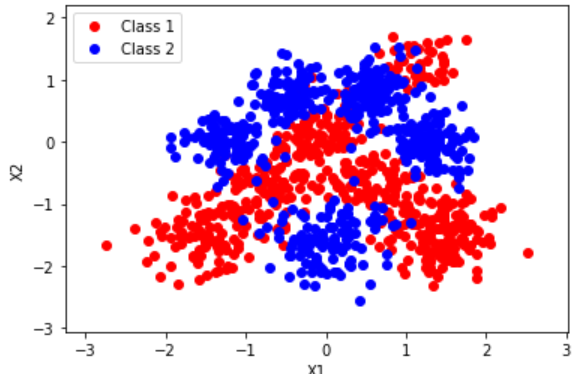
\includegraphics[width=70mm]{1.PNG}}
\subfigure[Training sets]{\label{fig:b}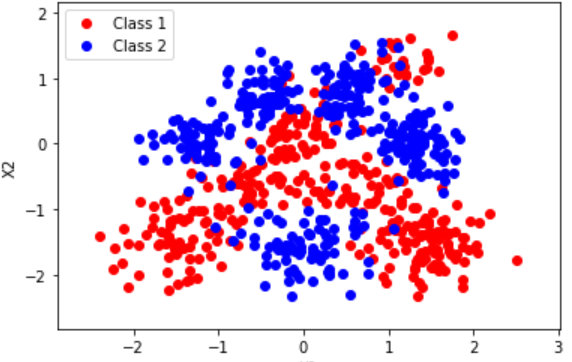
\includegraphics[width=70mm]{2.PNG}}
\caption{EDA}
\end{figure}
The data is then split into training and test sets, using existing $\text{train\_test\_split}()$ function provided by the $\text{sklearn.metrics}$ library, a split ratio of 70:30 is used as there is no need to cross validate the hyper parameters (a split ratio of 60:20:20 would have been used if a validation set is needed). A random seed is chosen to ensure the randomization step is reproducible (for debug and result sharing purposes). Figure shown in \ref{fig:b} is the plot of the training set, it is clear that the training set is representative of all datapoints.
\section{Python Implementation}
The code described in \ref{algo:grad} is implemented in python and is used to train the Logistic Classification method on the dataset.The red line from figure \ref{fig:c} shows the average log-likelihood obtained when the classifier is only trained on the raw input features. The predictions are visualized by adding probability contours to the plots made in figure \ref{fig:b}. It is clear that by using the linear model, it is impossible for the solution space to be reached. The final training and testing log-likelihoods per datapoint is 0.62 and -0.63 respectively. The fact that the testing error is slightly less than training error indicates that underfitting may be present. \\
\begin{figure}[htbp]
\centering     %%% not \center
\subfigure[All datapoints]{\label{fig:c}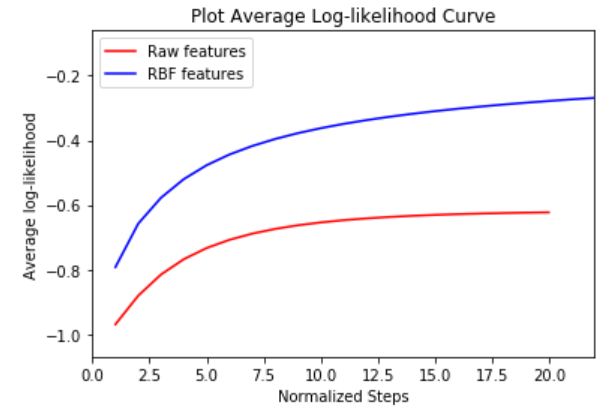
\includegraphics[width=70mm]{5.PNG}}
\subfigure[Training sets]{\label{fig:d}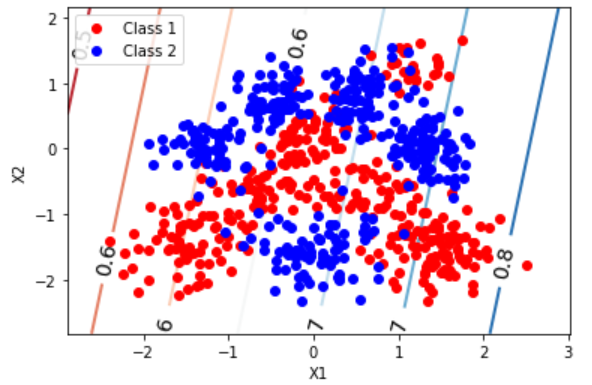
\includegraphics[width=70mm]{3.PNG}}
\caption{Training on raw input features}
\end{figure}
\begin{table}[htb]
\begin{tabular}{llll}
&                        & \multicolumn{2}{c}{predicted label, $\hat{y}$}                                      \\ \cline{3-4} 
& \multicolumn{1}{l|}{}  & \multicolumn{1}{c|}{0}                                                                     & \multicolumn{1}{c|}{1}                                                                     \\ \cline{2-4} 
\multicolumn{1}{c|}{\multirow{2}{*}{y}} & \multicolumn{1}{l|}{0} & \multicolumn{1}{l|}{$P(\hat{y}=0|y=0)$=0.752}                                            & \multicolumn{1}{l|}{\begin{tabular}[c]{@{}l@{}}$P(\hat{y}=0|y=1)$ = 0.321\end{tabular}} \\ \cline{2-4} 
\multicolumn{1}{c|}{}                   & \multicolumn{1}{l|}{1} & \multicolumn{1}{l|}{\begin{tabular}[c]{@{}l@{}}$P(\hat{y}=0|y=1)$ = 0.248\end{tabular}} & \multicolumn{1}{l|}{\begin{tabular}[c]{@{}l@{}}$P(\hat{y}=1|y=1)$ = 0.679\end{tabular}} \\ \cline{2-4} 
\end{tabular}
\label{tab:1}
\caption{Confusion matrix for raw features input}
\end{table}
The 2x2 confusion matrix is constructed through the standard $\text{confusion\_matrix}()$ function provided by the $\text{sklearn.metrics}$ library shown in table \ref{tab:1}, this table is obtained by setting no biase in the prediction threshold, i.e if the prediction probability is greater than 0.5, the output gets mapped to class label $\hat{y}=1$. The F1 score calculated from the confusion matrix is 0.715.
\section{Feature Expansion}
\label{sec:fet}
In order to reach the solution space, non-linearities are introduced to the input features. Instead of feature crossing, the inputs are expanded through a set of radial basis functions (RBFs) centred on the training datapoints. The $m+1$th feature of a datapoint therefore represents the amount of deviation of the datapoint from the $m$th datapoint in the training set, calculated as:
\begin{equation}
\hat{x}_{m+1}^{(n)} = exp\left(  -  \dfrac{1}{2l^2}   \sum_{d=1}^{2} (x_d^{(n)}  - x_d^{(m)})^2     \right)
\end{equation}
Where $l$ is a hyperparameter denoting the width of the radial basis function, as it is observed later, this parameter determines wether the model is overfitting or underfitting the data. Figure \ref{fig:rbf} shows different decision boundaries drawn by varying the width $l=\{0.01, 0.1, 1\}$, it is clear tha for $l=0.01, 0.1$ the decision boundaries are over complicated therefore resulting in an over-fitted model. On the contrary, when $l=1$, the decision boundries are too wide, resulting in an under-fitted model. The optimum parameter for $l$ therefore lies somewhere around 0.1 and 1, a grid search in space $\{l, \eta\}$ where $\eta$ is the learning rate, can be used to determine the close-to-optimum hyperparameters.

\begin{table}[htbp]
\begin{tabular}{llllllll}
                  & \textbf{train loss} & \textbf{test loss} & \textbf{$C_{00}$} & \textbf{$C_{01}$} & \textbf{$C_{10}$} & \textbf{$C_{11}$} & \textbf{$F1$} \\ \cline{2-8} 
\textbf{raw}      & -0.62               & -0.633             & 124               & 53                & 41                & 112               & 0.714         \\
\textbf{$l=0.01$} & -0.055              & -0.661             & 12                & 165               & 2                 & 151               & 0.385         \\
\textbf{$l=0.1$}  & -0.0786             & -0.31              & 154               & 23                & 17                & 136               & 0.874         \\
\textbf{$l=1$}    & -0.243              & -0.239             & 161               & 16                & 0                 & 143               & 0.92          \\
\textbf{$l=08$}   & -0.211              & -0.205             & 162               & 15                & 8                 & 145               & 0.93         
\end{tabular}
\caption{Performance table of RBF width}
\label{tab:rbf}
\end{table}
Table \ref{tab:rbf} shows the performance metrics with different RBF widths. Note that both the training and test set losses are in log-likelihood (closer to 0 the better), $C_{i,j}$ is a member in the \textbf{un-normalized} confusion matrix denoting $P(\hat{y}=i|y=j)$. Note that all RBF expansions except for when $l=0.01$ beat raw input features. When $l=0.01$, training loss is a lot less negative than test loss, indicating overfitting which is observed in figure \ref{fig:f}, which corresponds the extremely poor performance on the test set when $y=1$. Similar situation albeit less severe is observed when $l=0.1$. Test loss is slightly above the training loss when $l=1$, hence some degree of underfitting is present, this is validated in figure \ref{fig:h}. Through experimentation (grid search not implemented), the solution of $l=0.8$ seems to be close to optimum.

\begin{figure}[htbp]
\centering     %%% not \center
\subfigure[$l=0.01$]{\label{fig:f}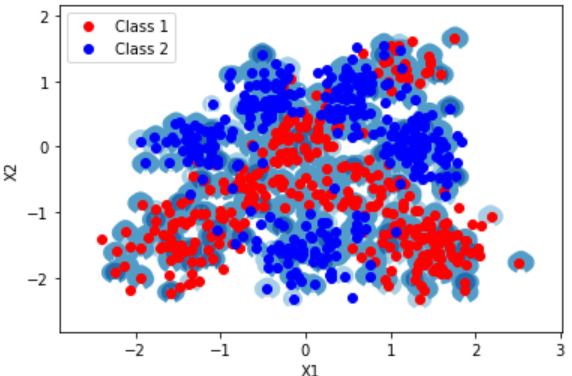
\includegraphics[width=70mm]{6.PNG}}
\subfigure[$l=0.1$]{\label{fig:g}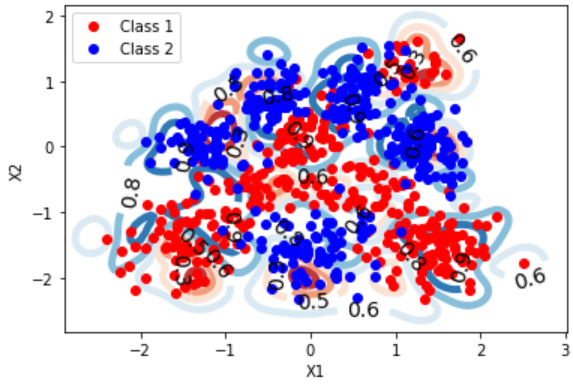
\includegraphics[width=70mm]{8.PNG}}
\subfigure[$l=1$]{\label{fig:h}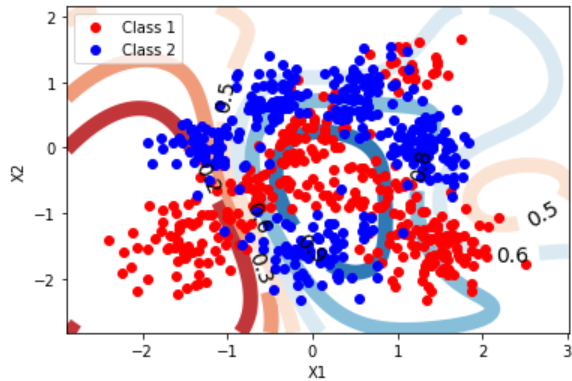
\includegraphics[width=70mm]{7.PNG}}
\caption{RBF features learning devision boundaries}
\label{fig:rbf}
\end{figure}

\section{Conclusion and Discussion}
The coursework investigated a Logistic Regression model, with gradient ascent derived from taking the gradient of log-likelihood of data generation, with respect to the parameters representing the weights of the input features. The aspects of a Logistic Regression model are demonstrated on a simple binary classification of two dimensional datapoints.\\ 
Without feature engineering, it is observed that linear combination of raw input features is unable to reach the solution space, caused by underfitting. RBF is used to add non linearities and expand the feature dimension, one hyper-parameter is the width of the RBF function. Significant overfitting is observed when the width is too low ($l=0.01$), some degree of underfitting is observed when the with is large ($l=1$). Overall, a F1 score of $93\%$ is achieved on the dataset using $l=0.8, \eta=0.001$, where $\eta$ is the learning rate. Logistic regression can therefore provide good estimation on classification problems.


\section{Appendix: Jupyter Notebook}
\begin{lstlisting}[language=Python]
#!/usr/bin/env python
# coding: utf-8

# # 3F8 Logistic Regression Lab
# #### *Submitted by Tom Lu xl402 on 1/17/2019*

# In[1]:

import numpy as np
from python_code import *
from sklearn.model_selection import train_test_split
from sklearn.metrics import confusion_matrix
from sklearn.metrics import f1_score

# ## EDA

# In[2]:

# Load data, X is the input featire matrix, y is the one-hot encoded label
X = np.loadtxt('X.txt')
y = np.loadtxt('y.txt')
print("X has shape: {}, y has shape: {}".format(X.shape, y.shape))


# **c) Using the given function *plot_data()*, the dataset is visualised in the two dimensional input space displaying each datapoint's class label**

# In[3]:

plot_data(X,y)

# Clearly this problem cannot be linearly seperated, feature crossings should be used (later on) to improve classification accuracy

# **d) Split the data into training and test sets**
# Using the *train_test_split()* function already provided by sklearn, with a fixed random seed to make the results reproducable each time, the test/train dataset ratio is set to be 33% V 67%, this is because our dataset is sufficiently large

# In[4]:

X_train, X_test, y_train, y_test = train_test_split(X, y, test_size=0.33, random_state=69)
# Visualize it just to be sure it is representative of the actual data set
plot_data(X_train,y_train)
print("X_train has shape: {}, y_train has shape: {}".format(X_train.shape, y_train.shape))

# **e) Transform the pseudocode from the perperation exercise into python code**


# Define sigmoid function
def sigmoid(x):
    return 1/(1+np.exp(-x))

def pad_bias(X):
    return np.append(np.ones((X.shape[0], 1)), X, axis = 1)

def logistic_regression(X_data, y_data, l_rate = 0.001, max_iter = 1000):
    
    loss = []
    # Add bias to training set
    X_data = pad_bias(X_data)
    
    # Initialize weights
    b = np.random.uniform(-1, 1, X_data.shape[1])

    for i in range (0, max_iter):
        # Compute sigmoid(Xb)
        y_pred = sigmoid(np.dot(X_data, b))
        
        # Compute log liklihood
        loss.append(compute_average_ll(X_data, y_data, b))
        
        # Weights update
        b = b + l_rate * np.dot(np.transpose(X_data), y_data-y_pred)
    return b, loss

# In[29]:
def plot_ll_2(ll, ll2):
    plt.figure()
    ax = plt.gca()
    plt.xlim(0, len(ll) + 2)
    plt.ylim(min(ll) - 0.1, max(ll2) + 0.1)
    ll2 = np.asarray(ll2)
    ax.plot(np.arange(1, len(ll) + 1), ll,'r-')
    ll2 = ll2.reshape(-1,len(ll)).mean(axis=1)
    ax.plot(np.arange(1, len(ll2) + 1), ll2,'b-')
    plt.legend(['Raw features', 'RBF features'], loc='upper left')
    plt.xlabel('Normalized Steps')
    plt.ylabel('Average log-likelihood')
    plt.title('Plot Average Log-likelihood Curve')
    plt.show()

# Report the average log likelihood after each training step

# In[26]:

b, loss_array = logistic_regression(X_train, y_train, 0.001, max_iter = 20)
plot_ll(loss_array)


# Visualise the predictions by adding probability contours to the plots made in part c)

# In[10]:

plot_predictive_distribution(X_train, y_train, b, predict_for_plot)

# Two helper functions which return the predicted label for given input features and parameters, if *thresh* is set to a value, then for all probabilities above the threshold, the label returns 1, otherwise 0.

# In[11]:


def predict_threshold(y_pred, thresh):
    y_pred[y_pred > thresh] = 1
    y_pred[y_pred <= thresh] = 0
    return y_pred

def predict_y(X_data, param, thresh = None):
    X_data = np.append(np.ones((X_data.shape[0], 1)), X_data, axis = 1)
    if thresh != None:
        return predict_threshold(sigmoid(np.dot(X_data, param)), thresh)
    else:
        return sigmoid(np.dot(X_data, param))

# Report the final traning and test log-likelihoods per datapoint.

# In[12]:

ll_train = compute_average_ll(pad_bias(X_train), y_train, b)
print("Final training log-likelihood: {}".format(ll_train))

ll_test = compute_average_ll(pad_bias(X_test), y_test, b)
print("Final test set log-likelihood: {}".format(ll_test))

# **f) For the test data, apply a threshold to the probabilistic predictions. Confusion matrix and f1 score are calculated**

y_pred = predict_y(X_test, b, 0.5)
c = confusion_matrix(y_test, y_pred)
f1 = f1_score(y_test, y_pred, average='macro')  
print("Test Set Confusion matrix: {}".format(c))
print("f1 score: {}".format(f1))

# **g) Expand the inputs through a set of RBFs centred on the training datapoints**

# In[241]:

def expand_inputs(l, X, Z):
    X2 = np.sum(X**2, 1)
    Z2 = np.sum(Z**2, 1)
    ones_Z = np.ones(Z.shape[ 0 ])
    ones_X = np.ones(X.shape[ 0 ])
    r2 = np.outer(X2, ones_Z) - 2 * np.dot(X, Z.T) + np.outer(ones_X, Z2)
    return np.exp(-0.5 / l**2 * r2)

rbf_kernel_size = 0.01
X_train_rbf = expand_inputs(rbf_kernel_size, X_train, X_train)

# Train the logistic classification model on the feature expanded inputs and display the new predictions

b_rbf, loss_array_rbf = logistic_regression(X_train_rbf, y_train, 0.01, max_iter = 2000)
plot_ll(loss_array_rbf)
loss_array_rbf[-1]

# In[244]:

plot_ll_2(loss_array,loss_array_rbf)

# In[175]:
def plot_predictive_distribution_expanded(X, y, b):
    xx, yy = plot_data_internal(X, y)
    ax = plt.gca()
    X_predict = np.concatenate((xx.ravel().reshape((-1, 1)),
                                yy.ravel().reshape((-1, 1))), 1)
    x_expanded = expand_inputs(rbf_kernel_size, X_predict, X_train)
    x_tilde = np.concatenate((x_expanded, np.ones((x_expanded.shape[ 0 ], 1 ))), 1)
    Z = logistic(np.dot(x_tilde, b))
    Z = Z.reshape(xx.shape)
    cs2 = ax.contour(xx, yy, Z, cmap = 'RdBu', linewidths = 5)
    plt.clabel(cs2, fmt = '%2.1f', colors = 'k', fontsize = 14)
    plt.show()

# Visualise the predictions using probability contours as in part e)

# In[176]:

plot_predictive_distribution_expanded(X_train, y_train, b_rbf)

# **h) Report the final training and test log-likelihoods per datapoint, the 2x2 confusion matricies are generated for rbf kernel size = {0.01, 0.1, 1}**

# In[170]:
X_test_rbf = expand_inputs(rbf_kernel_size, X_test, X_train)
y_pred = predict_y(X_test_rbf, b_rbf, 0.5)
c = confusion_matrix(y_test, y_pred)
f1 = f1_score(y_test, y_pred, average='macro')  
print("Test set confusion matrix: {}, kernel size is {}".format(c, rbf_kernel_size))
print("f1 score: {}".format(f1))

# kerne = 0.001, f1: 0.410; kernel = 1, f1:0.909; kernel = 0.1, f1:0.896

# In[245]:

def compute_average_ll_2(y, y_pred, w):
    return np.mean(y * np.log(y_pred)
                   + (1 - y) * np.log(1.0 - y_pred)) 
# In[246]:
X_test_rbf = expand_inputs(rbf_kernel_size, X_test, X_train)
y_pred_test = predict_y(X_test_rbf, b_rbf)
y_pred_train = predict_y(X_train_rbf, b_rbf)
ll_train = compute_average_ll_2(y_train, y_pred_train, b_rbf)
ll_test_1 = compute_average_ll_2(y_test, y_pred_test, b_rbf)
print(ll_train)
print(ll_test_1)
y_pred = predict_y(X_test_rbf, b_rbf, 0.5)

c = confusion_matrix(y_test, y_pred)
f1 = f1_score(y_test, y_pred, average='macro')  
print("Test set confusion matrix: {}, kernel size is {}".format(c, rbf_kernel_size))
print("f1 score: {}".format(f1))
\end{lstlisting}

\end{document}




















